\chapter*{监译者解说}
\phantomsection\addcontentsline{toc}{chapter}{监译者解说}
\markboth{监译者解说}{监译者解说}

% [原文 p.191]
K 理论是从线性代数再往前一步、一直通向现代几何最前沿的一条路，它是由向量丛的稳定等价类构成的一般上同调论。向量丛的稳定等价类就是超巨型矩阵的线性代数；既然线性化与稳定化是现代几何的基本策略，K 理论便在现代几何中无处不在。

本书是 Atiyah 教科书 \textit{K-theory} 的全译。原著以 1964 年 Atiyah 在哈佛大学授课、由 Anderson 记录的笔记为基础，1967 年由 W. A. Benjamin 公司出版 [13]，1989 年内容修订后由 Addison-Wesley 公司出版 [17]；另有俄文译本 [14]。本书以 1967 年版为底本译出。1967 年版与 1989 年版的差别见后文。翻译时先由译者川边治之译出全稿，再由监译者松尾审读内容；其间修正了若干轻微的数学错误与定理编号重复，并把部分记号改成现代的标准记号。

K 理论最好的入门书就是本书。学过线性代数与拓扑空间、正想着「接下来该学什么」而心潮澎湃的读者，务请一读。

\backsection{1. Atiyah 与 K 理论}
\para{1.1 关于 Atiyah}

Michael Francis Atiyah 1929 年 4 月 22 日生于伦敦，2019 年 1 月 11 日卒于爱丁堡。幼年在苏丹与埃及度过。1955 年在剑桥大学师从 Hodge 取得学位，在现代数学中活跃非凡，培养了众多优秀弟子。1966 年获 Fields 奖，2004 年与 Singer 共同获 Abel 奖。1990 年至 1995 年任伦敦皇家学会会长。关于更详细的履历，可参见网站 Celebratio Mathematica（\url{https://celebratio.org/Atiyah_MF/}）。顺带一提，Atiyah 似乎读作 /ati:a/。

\begin{center}
  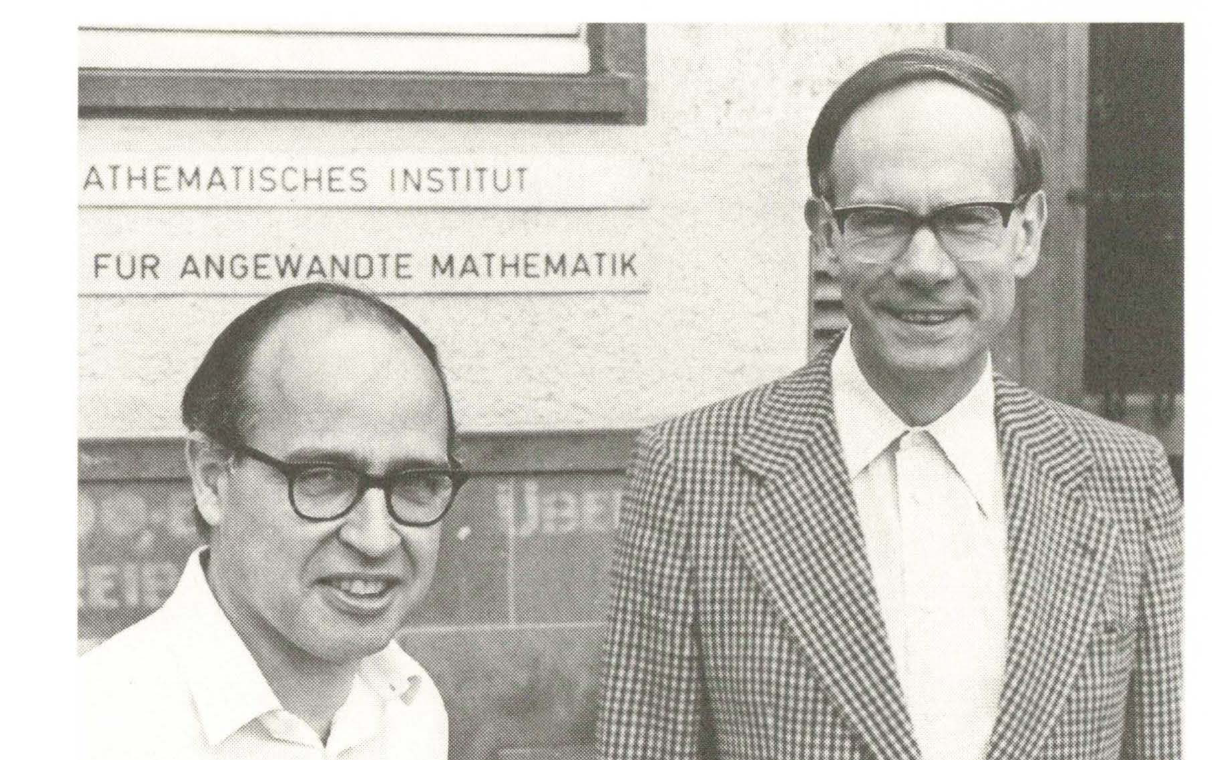
\includegraphics[width=0.62\textwidth]{figures/fig_atiyah_hirzebruch.png}

  \smallskip
  {\small Atiyah（左）与 Hirzebruch（右）（1977 年，波恩）\\
  照片提供：Archives of the Mathematisches Forschungsinstitut Oberwolfach}
\end{center}

% [原文 p.192]
Atiyah 的论文收在共七卷的全集 [16] 中。前五卷按领域整理，但尽管如此，大体上仍按时间顺序排列；配合各卷卷首的作者自注，可以窥见 Atiyah 数学的演变。主要业绩可举出：

\begin{itemize}[leftmargin=2em,itemsep=2pt]
\item Atiyah 与 Hirzebruch 引入作为一般上同调论的 K 理论 [20]
\item Atiyah--Singer 指标定理 [24--27] 与 Atiyah--Patodi--Singer 指标定理 [21--23]
\item Atiyah 与 Bott 关于 Riemann 面上的规范场论 [18]
\end{itemize}

此外，把以 Witten 为象征的现代物理广泛介绍给数学家，又反过来使物理学家理解现代数学的用处，从而促进数学与物理的交流，也是重要的工作。关于 Atiyah 的数学，悼念专辑 [37, 39, 52] 总结得极好。

\para{1.2 关于 K 理论}

K 理论的特征在于：

\begin{itemize}[leftmargin=2em,itemsep=2pt]
\item 它是一般上同调论之一；
\item 由向量丛的稳定等价类几何地构成；
\item Bott 周期性；
\item 经由 $J$ 群与指标定理，成为同伦论与大域分析的工具。
\end{itemize}

首先，K 理论是一般上同调论之一，具有 2.4 节所说明的完备体系，可用正合列与切除定理作具体计算。又，本书虽未说明，但借助 Chern 特征标与 Atiyah--Hirzebruch 谱序列，K 理论与上同调论联系在一起。

% [原文 p.193]
然而，各种一般上同调论并不是抽象地存在的。正如同调论与上同调论分别与子流形、微分形式相联系那样，K 群由向量丛几何地构成。Atiyah 尤其把 K 理论与向量丛的紧密关系看作自然之事，在各种一般上同调论中对 K 理论另眼相看；这一观点是本书的基调，以致 3.2 节竟把上同调群定义为 Adams 算子的特征空间。

进而，K 理论在同伦论与大域分析中有强有力的应用。例如 3.2 节所说明的，K 理论有 Adams 算子这一强力的上同调算子，它被用于球面上向量场的问题 [2] 与 Hopf 不变量问题 [9]，并通向第 3 章收尾的 $J(X)$ 研究 [3--7]。从同伦论的观点看，K 理论是 $V^{1}$ 周期的，位于 $V^{0}$ 周期的有理上同调论的下一个层级；再下一个层级则有椭圆上同调论与拓扑模形式等。K 理论是基于 $V^{n}$ 周期性的现代稳定同伦论中的试金石 [50]。又，如附录 A 所说明，K 群与 Fredholm 算子互为表里；在 Atiyah--Singer 指标定理的 K 理论证明中，Bott 周期性、Gysin 映射与椭圆型算子的指数浑然一体。

本书的主题是拓扑中的 K 理论，但在今天，K 理论的思想已越出拓扑而扩展：算子环的 K 理论 [32] 与代数 K 理论 [49] 分别在各自领域占据基本位置。与其他领域的 K 理论相对，拓扑中的 K 理论有时称为\emph{拓扑 K 理论}。而作为拓扑 K 理论本身的深化，还有扭 K 理论 [38, 55] 等。

% [原文 p.194]
历史上，1956 年 Bott 证明了他冠名的周期性，1957 年 Grothendieck 为推广 Hirzebruch--Riemann--Roch 定理而引入凝聚层的 K 群，这被视为开端。据全集第 2 卷的作者自注，本书定理 3.2.10 的 James 问题似乎成了他决心系统展开 K 理论的重大契机。1959 年 Atiyah 与 Hirzebruch 用 Bott 周期性把 Grothendieck 的 K 理论改编为一般上同调论。1962 年 Adams 用 K 理论解决了球面上向量场的问题，1963 年 Atiyah 与 Singer 发表指标定理的 K 理论证明，使 K 理论对现代几何的影响成为决定性的。进而，1964 年 Atiyah 与 Bott 发表周期性的初等证明，本书所依据的讲义也在此时讲授。顺带一提，K 理论的 K 来自表示 class（类）的德语词 Klasse，是 Grothendieck 命名的 [30]。最初他想用 class 的首字母写成 $C(X)$，但他研究过函数分析，意识到 $C(X)$ 会与连续函数空间混淆，于是改成了 $K(X)$。关于 K 理论的历史，Dieudonné 的 [36] 总结得极好。

\backsection{2. 预备知识与本书之后}
\para{2.1 预备知识}

开始读本书所必需的预备知识，只有拓扑空间与线性代数。例如并不需要懂同调与上同调。遇到未知术语时可靠的参考文献，有《岩波数学入门辞典》（青本和彦等编著，岩波书店，2005 年）与《岩波数学辞典第 4 版》（日本数学会编，岩波书店，2007 年）。网站 Algebraic Topology: A guide to literature（\url{http://pantodon.jp/}）也是信息的宝库。

拓扑空间方面，普通本科二年级课程所讲的程度就足够，只要具备紧 Hausdorff 空间的基本知识就能读下去。在 K 理论的语境中，推论 1.4.14 是紧 Hausdorff 空间最重要的性质。

% [原文 p.195]
线性代数方面需要稍进一步的知识。具体地说，1.2 节末尾列举的张量积、外代数等构造会本质地用到。线性代数就是「一点上的 K 理论」，例如教科书 [51]。环上的模，如 $K(X)$-模，也会出现，但知道定义就足够。

继续读下去还需要有限群表示论的初步知识，不过与本书并行学习即可。具体地说，只要 1.6 节能读，知道群作用、Schur 引理与不可约表示的分解就够。有限群表示论的经典名著有教科书 [53]。1.6 节开头对一般拓扑群陈述定义，但正文只处理有限群的情形。在 K 理论中考虑群作用，其意义超出单纯的推广。

又，1.2 节与 2.4 节出现范畴与函子，知道定义就够。2.2 节的 Bott 周期性证明中，Fejér 定理有教科书 [56]，取值于矩阵的函数的解析有教科书 [43]。关于 2.4 节提到的一般上同调论，从现代观点所作的解说有教科书 [45]。附录 A 需要 Fredholm 算子等 Hilbert 空间论的初步，教科书 [35] 易读。附录 B 的后半以上同调论与 Steenrod 算子为前提，内容稍进，初读时或许可以跳过。附录 C 处理的 Clifford 代数与 $KO$、$KR$ 理论，在论文 [19] 与教科书 [46] 中有更详细的处理。

\para{2.2 本书之后}

读完本书之后，无论如何都建议去翻一翻 Atiyah 全集第 2 卷，信手乱读。例如先读全集论文第 28 号 [20]，既可复习本书，又能新学 Chern 特征标与 Atiyah--Hirzebruch 谱序列。本书 2.7 节强调：把 Thom 同构定理推广到 $G$-向量丛需要真正的新手法。全集论文第 46 号 [15] 的主题正是这种新手法，即椭圆型偏微分算子的指数。第 3 卷与第 4 卷还可以从指标定理的观点

% [原文 p.196]
学习 K 理论。

从与本书不同的角度学习 K 理论也好。K 理论的教科书还有 Hirzebruch 的 [8, (20)] 与 Bott 的 [34]，对照阅读可以品味三位创始人各自不同的视角，意味深长。Karoubi 的教科书 [42] 阐明了 Clifford 代数在 K 理论中的作用，并与发端于 Kitaev [44] 的拓扑绝缘体分类相关联。又，综述 [10, 11] 很好地总结了 K 理论的全貌。

\backsection{3. 正文补注}
\para{3.1 1967 年版与 1989 年版的差别}

1989 年版除了修正轻微的数学错误，第 2 章前半还有改订，尤其 Bott 周期性的证明被大幅改写。这里说明第 2 章的变更点。

1989 年版的 2.1 节加入了 K 群的同伦论定义。映射 $\Vect_{n}(X)\to\Vect_{n+1}(X)$ 由与平凡线丛的直和来定义。此时，由稳定等价性的定义，对紧空间 $X$ 有
\[
  \tilde K(X)\cong\varinjlim_{n}\Vect_{n}(X).
\]
从而，对分类空间 $BU:=\varinjlim_{n}\bigl(\varinjlim_{m}G_{n}(\C^{m})\bigr)$，结合定理 1.4.15 可得
\[
  \tilde K(X)\cong\varinjlim_{n}\Vect_{n}(X)\cong\varinjlim_{n}\bigl[X,\varinjlim_{m}G_{n}(\C^{m})\bigr]\cong[X,BU].
\]
同样，对紧空间 $X$ 也可知
\[
  K(X)\cong[X,\Z\times BU]
\]
成立。又，对无限酉群 $U:=\varinjlim_{n}U(n)$，把引理 2.4.6 换个说法，便是
\[
  \tilde K(S(X))\cong[X,U].
\]

% [原文 p.197]
但这从同伦等价 $U\sim\Omega BU$ 也能看出。一般地，
\[
  K^{-n}(X)\cong[X,\Omega^{n}BU]\cong[X,\Omega^{n-1}U]
\]
成立。

又，1967 年版的 2.4 节在 1989 年版中变成 §2.2 \textit{Elementary properties}，没有本质差别。1967 年版中关于一般上同调论的注意在 1989 年版被删去，这或许表示一般上同调论这一领域的成熟。

1989 年版的 2.3 节说明 Bott 周期性。这是 1967 年版与 1989 年版最大的差异。Bott 的 Bott 周期性证明 [33] 中构造了具体嵌入
\[
  \beta_{n}\colon G_{n}(\C^{2n})=\frac{U(n)}{U(n)\times U(n)}\to\Omega U(2n),
\]
并通过考虑 $\Omega U(2n)$ 上的 Morse 理论，证明 $n\to\infty$ 的极限给出同伦等价映射
\[
  \beta\colon\Z\times BU\to\Omega U.
\]
如上所述，$K(X)\cong[X,\Z\times BU]$ 且 $K^{-2}(X)\cong[X,\Omega U]$，故映射 $\beta$ 导出同构 $K(X)\cong K^{-2}(X)$。要证明 $\beta\colon\Z\times BU\to\Omega U$ 是同构，也可以直接构造逆映射
\[
  \alpha\colon\Omega U\to\Z\times BU.
\]
进而由定理 A.1，族的指数映射
\[
  \operatorname{index}\colon\mathcal{F}\to\Z\times BU
\]
给出同伦等价。因此，为证明 Bott 周期性，只需构造映射
\[
  \alpha'\colon\Omega U\to\mathcal{F},
\]
使合成 $\operatorname{index}\circ\alpha'$ 成为同伦等价即可。直接构造这种 $\alpha'$ 的方法之一就是 Toeplitz 映射。

% [原文 p.198]
详见论文 [15]。

1989 年版的 Bott 周期性证明，就是论文 [15] 第 7 节 \textit{Comparison with elementary proof} 中作为 method (2A) 提到的内容。首先用 Laurent 多项式把 Toeplitz 映射作有限维近似，从而不经由 Fredholm 算子的空间 $\mathcal{F}$，而构造映射
\[
  \alpha\colon K(S^{2}\times X)\to K(X).
\]
又，上述 Bott 的映射 $\beta$ 与由 Bott 元 $([H]-1)\in K^{-2}(X)$ 的乘法给出的映射
\[
  \beta\colon K(X)\to K^{-2}(X)
\]
本质相同，这容易看出。然后利用 Atiyah 的旋转技巧 [15, Proposition (1.5)]，可证 $\alpha$ 是 $\beta$ 的逆映射。这大概是 Bott 周期性证明的一种极致。另，本书及 1967 年版中的 $\nu$ 与 $\mu$ 就是上面的 $\alpha$ 与 $\beta$。

1989 年版 2.4 节的内容与 1967 年版 2.3 节相同。2.5 节以后两者没有本质差异。

\para{3.2 第 3 章的背景及其后的发展}

第 3 章解说 K 理论的上同调算子及其应用。这里补几条文献。

关于 3.1 节的外幂算子，另见论文 [12, 28]。$\dim_{K}$ 也称几何维数（geometric dimension），论文 [12] 把它应用于实射影空间到欧氏空间的嵌入问题。

3.2 节处理 Adams 算子及其应用。定理 3.2.3 是「Hopf 不变量 1 的问题」，原论文为 [9]。此问题原本由 Adams [1] 运用上同调论的高次上同调算子解决，而 Atiyah 与 Adams 仅用 K 理论的一次算子给出了简洁的另证。又，Adams 论文 [1] 开头列举了相关问题，可作参考。像命题 3.2.6 那样把上同调群刻画为 Adams 算子的特征空间

% [原文 p.199]
一事，可参见论文 [9]。定理 3.2.10 是「James 问题」，原论文为 [29]，是球面上向量场问题 [2] 在复数情形的类比。又，如上所述，这个 James 问题似乎成了系统展开 K 理论的重大契机。最后的 $e$ 不变量参见论文 [6, Section 7]。

关于本书收尾的 3.3 节 $J(X)$，参见 Adams 的连作 [3--7]。论文 [3] 的 CONJECTURE (1.2) 曾被称为 Adams 猜想，现今已经解决 [31, 40, 47, 48, 54]。又，与 $J(X)$ 相关的群 $J'(X)$ 在四维流形论中有精彩的应用 [41]。这些证明以及其中展开的想法，无一不深刻。

撰写本文时，承蒙五味清纪、立川裕二、玉木大、深谷英则、古田干雄、前川拓海、森晃纪、森田阳介、横山广美、François Rigal 各位惠赐意见；编辑大桥耕先生对本书自始至终予以照顾。谨此致谢。

% [Tutor Note: 本节致谢名单的日文名字 OCR 有若干不可靠处（如「五味消紀」「森晃紀」），译文按 K 理论与相关领域通行写法录为「五味清纪」「森晃纪」；若与原书不符，以原书扫描页为准。]

\section*{参考文献}
\addcontentsline{toc}{section}{参考文献}
\begingroup
\small
\noindent [1] J. F. Adams, `On the non-existence of elements of Hopf invariant one', \textit{Ann. of Math.} \textbf{72}(2) (1960) 20--104.

\noindent [2] J. F. Adams, `Vector fields on spheres', \textit{Ann. of Math.} \textbf{75}(2) (1962) 603--632.

\noindent [3] J. F. Adams, `On the groups $J(X)$. I', \textit{Topology} \textbf{2} (1963) 181--195.

\noindent [4] J. F. Adams, `On the groups $J(X)$. II', \textit{Topology} \textbf{3} (1965) 137--171.

\noindent [5] J. F. Adams, `On the groups $J(X)$. III', \textit{Topology} \textbf{3} (1965) 193--222.

\noindent [6] J. F. Adams, `On the groups $J(X)$. IV', \textit{Topology} \textbf{5} (1966) 21--71.

\noindent [7] J. F. Adams, `Correction to: ``On the groups $J(X)$. IV''', \textit{Topology} \textbf{7} (1968) 331.

\noindent [8] J. F. Adams, \textit{Algebraic topology: a student's guide}, London Mathematical Society Lecture Note Series, No. 4, Cambridge University Press, London--New York, 1972.

% [原文 p.200]
\noindent [9] J. F. Adams and M. F. Atiyah, `K-theory and the Hopf invariant', \textit{Quart. J. Math. Oxford Ser.} \textbf{17}(2) (1966) 31--38.

\noindent [10] 荒木捷朗「位相的 $K$ 理論 I」『数学』\textbf{22}(1) (1970) 60--76.

\noindent [11] 荒木捷朗「位相的 $K$ 理論 II」『数学』\textbf{23}(4) (1971) 272--292.

\noindent [12] M. F. Atiyah, `Immersions and embeddings of manifolds', \textit{Topology} \textbf{1} (1962) 125--132.

\noindent [13] M. F. Atiyah, \textit{K-theory}, W. A. Benjamin, Inc., New York--Amsterdam, 1967. Notes by D. W. Anderson.

\noindent [14] M. At'ja, \textit{Lektsii po K-teorii}, Translated from the English by V. M. Bukhshtaber, V. N. Resetnikov, and D. B. Fuks; Edited by A. A. Kirillov, Izdat. ``Mir'', Moscow, 1967.

\noindent [15] M. F. Atiyah, `Bott periodicity and the index of elliptic operators', \textit{Quart. J. Math. Oxford Ser.} \textbf{19}(2) (1968) 113--140.

\noindent [16] M. F. Atiyah, \textit{Michael Atiyah Collected Works.} Vol. 1--7, The Clarendon Press, Oxford University Press, New York, 1988--2014.

\noindent [17] M. F. Atiyah, \textit{K-theory}, Addison-Wesley Publishing Company, Redwood City, CA, 1989. Notes by D. W. Anderson.

\noindent [18] M. F. Atiyah and R. Bott, `The Yang-Mills equations over Riemann surfaces', \textit{Philos. Trans. Roy. Soc. London Ser. A} \textbf{308}(1505) (1983) 523--615.

\noindent [19] M. F. Atiyah, R. Bott, and A. Shapiro, `Clifford modules', \textit{Topology} \textbf{3} (1964), no. suppl. 1, 3--38.

\noindent [20] M. F. Atiyah and F. Hirzebruch, \textit{Vector bundles and homogeneous spaces}, Proc. Sympos. Pure Math., Vol. III, American Mathematical Society, Providence, R.I., 1961, 7--38.

\noindent [21] M. F. Atiyah, V. K. Patodi, and I. M. Singer, `Spectral asymmetry and Riemannian geometry. I', \textit{Math. Proc. Cambridge Philos. Soc.} \textbf{77}(1) (1975) 43--69.

\noindent [22] M. F. Atiyah, V. K. Patodi, and I. M. Singer, `Spectral asymmetry and Riemannian geometry. II', \textit{Math. Proc. Cambridge Philos. Soc.} \textbf{78}(3) (1975) 405--432.

\noindent [23] M. F. Atiyah, V. K. Patodi, and I. M. Singer, `Spectral asymmetry and Riemannian geometry. III', \textit{Math. Proc. Cambridge Philos. Soc.} \textbf{79}(1) (1976) 71--99.

\noindent [24] M. F. Atiyah and I. M. Singer, `The index of elliptic operators. I', \textit{Ann. of Math.}

% [原文 p.201]
\noindent \textbf{87}(3) (1968) 484--530.

\noindent [25] M. F. Atiyah and I. M. Singer, `The index of elliptic operators. III', \textit{Ann. of Math.} \textbf{87}(3) (1968) 546--604.

\noindent [26] M. F. Atiyah and I. M. Singer, `The index of elliptic operators. IV', \textit{Ann. of Math.} \textbf{93}(1) (1971) 119--138.

\noindent [27] M. F. Atiyah and I. M. Singer, `The index of elliptic operators. V', \textit{Ann. of Math.} \textbf{93}(1) (1971) 139--149.

\noindent [28] M. F. Atiyah and D. O. Tall, `Group representations, $\lambda$-rings and the $J$-homomorphism', \textit{Topology} \textbf{8} (1969) 253--297.

\noindent [29] M. F. Atiyah and J. A. Todd, `On complex Stiefel manifolds', \textit{Proc. Cambridge Philos. Soc.} \textbf{56} (1960) 342--353.

\noindent [30] A. Bak, Editorial. \textit{K-Theory} \textbf{1}(1) (1987) 1--4.

\noindent [31] J. C. Becker and D. H. Gottlieb, `The transfer map and fiber bundles', \textit{Topology} \textbf{14} (1975) 1--12.

\noindent [32] B. Blackadar, \textit{K-theory for operator algebras}, Cambridge University Press, Cambridge, 1998.

\noindent [33] R. Bott, `The stable homotopy of the classical groups', \textit{Ann. of Math.} \textbf{70}(2) (1959) 313--337.

\noindent [34] R. Bott, \textit{Lectures on $K(X)$}, Mathematics Lecture Note Series, W. A. Benjamin, Inc., New York--Amsterdam, 1969.

\noindent [35] 黒田成俊『関数解析』共立出版 1980.

\noindent [36] J. Dieudonné, \textit{A history of algebraic and differential topology 1900--1960}, Modern Birkhäuser Classics, Birkhäuser Boston, Ltd., Boston, MA, 2009. Reprint of the 1989 edition.

\noindent [37] S. Donaldson, `Atiyah's work on holomorphic vector bundles and gauge theories', \textit{Bull. Amer. Math. Soc. (N.S.)} \textbf{58}(4) (2021) 567--610.

\noindent [38] P. Donovan and M. Karoubi, \textit{Graded Brauer groups and K-theory with local coefficients}, Inst. Hautes Études Sci. Publ. Math., \textbf{38} (1970) 5--25.

\noindent [39] D. S. Freed, `The Atiyah--Singer index theorem', \textit{Bull. Amer. Math. Soc. (N.S.)} \textbf{58}(4) (2021) 517--566.

\noindent [40] E. M. Friedlander, `Fibrations in étale homotopy theory', \textit{Inst. Hautes Études Sci. Publ. Math.} \textbf{42} (1973) 5--46.

\noindent [41] M. Furuta, `Monopole equation and the $\frac{11}{8}$-conjecture', \textit{Math. Res. Lett.} \textbf{8}(3) (2001) 279--291.

\noindent [42] M. Karoubi, \textit{K-theory}, Classics in Mathematics, Springer-Verlag, Berlin,

% [原文 p.202]
\noindent 2008. An introduction; Reprint of the 1978 edition.

\noindent [43] 加藤敏夫（丸山徹訳）『行列の摂動』丸善出版 2012.

\noindent [44] A. Kitaev, \textit{Periodic table for topological insulators and superconductors}, AIP Conference Proceedings \textbf{1134} (2009) 22--30.

\noindent [45] 河野明·玉木大『一般コホモロジー』岩波書店, 2008.

\noindent [46] H. B. Lawson Jr. and M.-L. Michelsohn, \textit{Spin geometry}, Princeton Mathematical Series, vol. 38, Princeton University Press, Princeton, NJ, 1989.

\noindent [47] D. G. Quillen, `Some remarks on étale homotopy theory and a conjecture of Adams', \textit{Topology} \textbf{7} (1968) 111--116.

\noindent [48] D. Quillen, `The Adams conjecture', \textit{Topology} \textbf{10} (1971) 67--80.

\noindent [49] D. Quillen, \textit{Higher algebraic K-theory: I}. In: H. Bass (eds.), \textit{Higher K-Theories}, Springer, Berlin, Heidelberg, 1973.

\noindent [50] D. C. Ravenel, \textit{Nilpotence and periodicity in stable homotopy theory}, Princeton University Press, Princeton, NJ, 1992. Appendix C by Jeff Smith.

\noindent [51] 斎藤毅『線形代数の世界』東京大学出版会, 2007.

\noindent [52] G. Segal, `Michael Atiyah's work in algebraic topology', \textit{Bull. Amer. Math. Soc. (N.S.)} \textbf{58}(4) (2021) 481--516.

\noindent [53] J.-P. セール（岩堀長慶·横沼健雄訳）『有限群の線型表現』岩波書店, 1974.

\noindent [54] D. Sullivan, `Genetics of homotopy theory and the Adams conjecture', \textit{Ann. of Math.} \textbf{100}(2) (1974) 1--79.

\noindent [55] J. Rosenberg, `Continuous-trace algebras from the bundle theoretic point of view', \textit{J. Austral. Math. Soc. Ser. A} \textbf{47}(3) (1989) 368--381.

\noindent [56] 高橋陽一郎『実関数とフーリエ解析』岩波書店, 2006.
\endgroup
% CHUNK kaisetsu DONE
